\documentclass[twoside]{book}

% Packages required by doxygen
\usepackage{fixltx2e}
\usepackage{calc}
\usepackage{doxygen}
\usepackage[export]{adjustbox} % also loads graphicx
\usepackage{graphicx}
\usepackage[utf8]{inputenc}
\usepackage{makeidx}
\usepackage{multicol}
\usepackage{multirow}
\PassOptionsToPackage{warn}{textcomp}
\usepackage{textcomp}
\usepackage[nointegrals]{wasysym}
\usepackage[table]{xcolor}

% Font selection
\usepackage[T1]{fontenc}
\usepackage[scaled=.90]{helvet}
\usepackage{courier}
\usepackage{amssymb}
\usepackage{sectsty}
\renewcommand{\familydefault}{\sfdefault}
\allsectionsfont{%
  \fontseries{bc}\selectfont%
  \color{darkgray}%
}
\renewcommand{\DoxyLabelFont}{%
  \fontseries{bc}\selectfont%
  \color{darkgray}%
}
\newcommand{\+}{\discretionary{\mbox{\scriptsize$\hookleftarrow$}}{}{}}

% Page & text layout
\usepackage{geometry}
\geometry{%
  a4paper,%
  top=2.5cm,%
  bottom=2.5cm,%
  left=2.5cm,%
  right=2.5cm%
}
\tolerance=750
\hfuzz=15pt
\hbadness=750
\setlength{\emergencystretch}{15pt}
\setlength{\parindent}{0cm}
\setlength{\parskip}{3ex plus 2ex minus 2ex}
\makeatletter
\renewcommand{\paragraph}{%
  \@startsection{paragraph}{4}{0ex}{-1.0ex}{1.0ex}{%
    \normalfont\normalsize\bfseries\SS@parafont%
  }%
}
\renewcommand{\subparagraph}{%
  \@startsection{subparagraph}{5}{0ex}{-1.0ex}{1.0ex}{%
    \normalfont\normalsize\bfseries\SS@subparafont%
  }%
}
\makeatother

% Headers & footers
\usepackage{fancyhdr}
\pagestyle{fancyplain}
\fancyhead[LE]{\fancyplain{}{\bfseries\thepage}}
\fancyhead[CE]{\fancyplain{}{}}
\fancyhead[RE]{\fancyplain{}{\bfseries\leftmark}}
\fancyhead[LO]{\fancyplain{}{\bfseries\rightmark}}
\fancyhead[CO]{\fancyplain{}{}}
\fancyhead[RO]{\fancyplain{}{\bfseries\thepage}}
\fancyfoot[LE]{\fancyplain{}{}}
\fancyfoot[CE]{\fancyplain{}{}}
\fancyfoot[RE]{\fancyplain{}{\bfseries\scriptsize Generated by Doxygen }}
\fancyfoot[LO]{\fancyplain{}{\bfseries\scriptsize Generated by Doxygen }}
\fancyfoot[CO]{\fancyplain{}{}}
\fancyfoot[RO]{\fancyplain{}{}}
\renewcommand{\footrulewidth}{0.4pt}
\renewcommand{\chaptermark}[1]{%
  \markboth{#1}{}%
}
\renewcommand{\sectionmark}[1]{%
  \markright{\thesection\ #1}%
}

% Indices & bibliography
\usepackage{natbib}
\usepackage[titles]{tocloft}
\setcounter{tocdepth}{3}
\setcounter{secnumdepth}{5}
\makeindex

% Hyperlinks (required, but should be loaded last)
\usepackage{ifpdf}
\ifpdf
  \usepackage[pdftex,pagebackref=true]{hyperref}
\else
  \usepackage[ps2pdf,pagebackref=true]{hyperref}
\fi
\hypersetup{%
  colorlinks=true,%
  linkcolor=blue,%
  citecolor=blue,%
  unicode%
}

% Custom commands
\newcommand{\clearemptydoublepage}{%
  \newpage{\pagestyle{empty}\cleardoublepage}%
}

\usepackage{caption}
\captionsetup{labelsep=space,justification=centering,font={bf},singlelinecheck=off,skip=4pt,position=top}

%===== C O N T E N T S =====

\begin{document}

% Titlepage & ToC
\hypersetup{pageanchor=false,
             bookmarksnumbered=true,
             pdfencoding=unicode
            }
\pagenumbering{alph}
\begin{titlepage}
\vspace*{7cm}
\begin{center}%
{\Large py\+E\+B\+F\+Gen \\[1ex]\large 0.\+2.\+0 }\\
\vspace*{1cm}
{\large Generated by Doxygen 1.8.13}\\
\end{center}
\end{titlepage}
\clearemptydoublepage
\pagenumbering{roman}
\tableofcontents
\clearemptydoublepage
\pagenumbering{arabic}
\hypersetup{pageanchor=true}

%--- Begin generated contents ---
\chapter{ebfgen}
\label{md_README}
\Hypertarget{md_README}
Python batch file generator for use with the F\+CC E\+BF system.

F\+CC Documentation can be found at\+: \href{https://www.fcc.gov/wireless/systems-utilities/uls-electronic-batch-filing}{\tt https\+://www.\+fcc.\+gov/wireless/systems-\/utilities/uls-\/electronic-\/batch-\/filing}

This should work cross-\/platform; however my main development environment is Linux. If you try on Mac / Windows and find platform-\/specific bugs, please let me know.

$\ast$$\ast$ Version 0.\+2 base $\ast$$\ast$ Version 0.\+2 represents a pretty big sway from version 0.\+1, in hopes that it\textquotesingle{}ll make things considerably more maintainable. This version should be considered unstable, and should not be used.

\subsection*{Requirements}


\begin{DoxyItemize}
\item Python 3.\+5.\+3+
\item python3-\/tk
\end{DoxyItemize}

\subsection*{Installation / Execution}

\subsubsection*{Linux}


\begin{DoxyItemize}
\item Clone from github\+: {\ttfamily git clone \href{https://github.com/dpurgert/pyebfgen.git}{\tt https\+://github.\+com/dpurgert/pyebfgen.\+git}}
\item (Optional) add execute permissions\+: {\ttfamily chmod u+x ebfgen.\+py}
\item Run with {\ttfamily python3 ebfgen.\+py}; or if you added execute permissions, {\ttfamily ./ebfgen.py}
\end{DoxyItemize}

\subsubsection*{Windows}


\begin{DoxyItemize}
\item Install Python3 (as of writing, 3.\+8.\+5 is current)
\begin{DoxyItemize}
\item Python can be downloaded by going to \href{https://www.python.org/downloads/}{\tt https\+://www.\+python.\+org/downloads/}
\end{DoxyItemize}
\item Download Zip archive of this repository
\item Unzip to your prefered location (e.\+g. Desktop)
\item Double-\/click \char`\"{}ebfgen.\+py\char`\"{}
\end{DoxyItemize}

\subsection*{changelog}

v 0.\+1.\+0 -\/ Stable Beta
\begin{DoxyItemize}
\item Should be stable now. Future patches, etc. based on user experience requests
\end{DoxyItemize}

v. 0.\+0.\+16 -\/ version string
\begin{DoxyItemize}
\item broke the version string up into individual vars.
\end{DoxyItemize}

v 0.\+0.\+15 -\/ UI Fixes
\begin{DoxyItemize}
\item Force callsign to uppercase
\item Zero-\/pad the F\+RN (if provided) to 10 digits
\item Remove formatting (parenthesis, dashes, etc.) from S\+SN, Phone Number, etc.
\item Limit name fields to lengths imposed by F\+CC
\item Limit mailing address fields to lengths imposed by F\+CC
\item Updated user guide for readability \& noted changes.
\end{DoxyItemize}

v 0.\+0.\+14 -\/ Added missing applicant field
\begin{DoxyItemize}
\item Added the name suffix field back into the application.
\item Tested...present and works.
\item Moved the callsign entry box to right side of same row.
\end{DoxyItemize}

v 0.\+0.\+13 -\/ Updated applicant interface
\begin{DoxyItemize}
\item Updated interface to follow the 605 form.
\end{DoxyItemize}

v 0.\+0.\+12 -\/ Update regional ID
\begin{DoxyItemize}
\item Allow lowercase region I\+Ds
\end{DoxyItemize}

v 0.\+0.\+11 -\/ Fix V\+EC \& Session Numbers G\+UI
\begin{DoxyItemize}
\item Fixed the interface to make it easier for the user to separate session date/location from actual numbers.
\item Moved the Regional Identifier to a location separating it from the remaining slots for organizational purposes.
\end{DoxyItemize}

v 0.\+0.\+10 -\/ Fix C\+R\+LF
\begin{DoxyItemize}
\item C\+R\+LF got eaten somewhere. Replacing it
\end{DoxyItemize}

v 0.\+0.\+9 -\/ Default Filename
\begin{DoxyItemize}
\item Added region code to V\+EC form
\item Added default filename as (V\+EC + mmdd + Region Code + counter).dat
\item Applicant data is cleared on save
\item file counter incremented on save. Can be set in V\+EC info form if necessary. Zero padding the number is automatic, if required
\item \char`\"{}working\char`\"{} output frame seems to have visual artifacts after reset. This is just a visual bug in the program, and does not affect output files.
\end{DoxyItemize}

v 0.\+0.\+8 -\/ Force V\+EC Code case
\begin{DoxyItemize}
\item V\+EC Code will always be stored capitalized.
\end{DoxyItemize}

v 0.\+0.\+7 -\/ Embed G\+NU Public Liense
\begin{DoxyItemize}
\item Embedded the G\+NU General Public License statement within source code.
\end{DoxyItemize}

v 0.\+0.\+6 -\/ Updated response processing
\begin{DoxyItemize}
\item Stick edited response file data into \char`\"{}applicant info\char`\"{} pane after importing.
\item Added button to clear frame on click.
\item NB\+: Frame data has no bearing on output file order. VE Header is A\+L\+W\+A\+YS first, and A\+L\+W\+A\+YS followed in \mbox{[}0 .. n\mbox{]} order for VA records.
\end{DoxyItemize}

v 0.\+0.\+5 -\/ Input verification
\begin{DoxyItemize}
\item verify input for S\+S\+N/\+F\+RN fields
\item verify input for Basic Qualification Question
\end{DoxyItemize}

v 0.\+0.\+4 -\/ Response Processing
\begin{DoxyItemize}
\item File menu cleanup
\item Response file conversion to comma-\/separated
\end{DoxyItemize}

v 0.\+0.\+3 -\/ Rename
\begin{DoxyItemize}
\item rename ulsbatch.\+py to ebfgen.\+py
\end{DoxyItemize}

v 0.\+0.\+2 -\/ Cosmetic modifications
\begin{DoxyItemize}
\item Changed menu names to adequately reflect information collected from the 605 form.
\item Made the menu entries more compact for the Individual Amateur radio license data entry window for smaller screens.
\end{DoxyItemize}

v 0.\+0.\+1 -\/ Initial alpha
\begin{DoxyItemize}
\item V\+EC / Test data set via File -\/$>$ VE
\item Add applicant data via File -\/$>$ VA
\begin{DoxyItemize}
\item \char`\"{}\+Standard\char`\"{} Applicant form assumes / hardcodes certain values
\item \char`\"{}\+Extended\char`\"{} applicant data also available, corresponds directly to F\+CC document. 
\end{DoxyItemize}
\end{DoxyItemize}
\chapter{Regional Identifier Listing}
\label{md_rid}
\Hypertarget{md_rid}
\subsection*{Here is the master list of regional identifiers, required to generate the session filename\+:}

-\/\+Letter-\/ Location / Region

-- A --- Aleutians East Borough \mbox{[}Alaska\mbox{]}

-- B --- Anchorage \mbox{[}Alaska\mbox{]}

-- C --- Bush (Remote) Alaska; all areas in Alaska that are N\+OT inside a borough

-- D --- Call District 0 (Lower 48)

-- E --- Call District 1 (Lower 48)

-- F --- Call Districts 2 and 3 (Lower 48)

-- G --- Call District 4 (Lower 48)

-- H --- Call Districts 5, 8 and 9 (Lower 48)

-- I --- Call District 6 (Lower 48)

-- J --- Call District 7 (Lower 48)

-- K --- City and Borough of Juneau \mbox{[}Alaska\mbox{]}

-- L --- City and Borough of Sitka \mbox{[}Alaska\mbox{]}

-- M --- Denali Borough \mbox{[}Alaska\mbox{]}

-- N --- Fairbanks North Star Borough \mbox{[}Alaska\mbox{]}

-- O --- Haines Borough \mbox{[}Alaska\mbox{]}

-- P --- Kenai Peninsula Borough \mbox{[}Alaska\mbox{]}

-- Q --- Ketchikan Gateway Borough \mbox{[}Alaska\mbox{]}

-- R --- Kodiak Island Borough \mbox{[}Alaska\mbox{]}

-- S --- Lake and Peninsula Borough \mbox{[}Alaska\mbox{]}

-- T --- Matanuska-\/\+Susitna Borough \mbox{[}Alaska\mbox{]}

-- U --- North Slope / Northwest Arctic Boroughs \mbox{[}Alaska\mbox{]}

-- V --- Petersburg Borough \mbox{[}Alaska\mbox{]}

-- W --- Skagway Borough \mbox{[}Alaska\mbox{]}

-- X --- Wrangell Borough \mbox{[}Alaska\mbox{]}

-- Y --- Yakutat Borough \mbox{[}Alaska\mbox{]}

-- Z --- Remote and International Sessions

-- a --- Puerto Rico and U.\+S. Virgin Islands

-- b --- American Samoa, Guam, Hawaii and Northern Mariana Islands 
\chapter{py\+E\+B\+F\+Gen Guide}
\label{md_UserGuide}
\Hypertarget{md_UserGuide}
$\ast$$\ast$ Version 0.\+2 base $\ast$$\ast$ Version 0.\+2 represents a pretty big sway from version 0.\+1, in hopes that it\textquotesingle{}ll make things considerably more maintainable. This version should be considered unstable, and should not be used.

\subsection*{Overview}

This guide is intended to give you a quick overview of how to use the py\+E\+B\+F\+Gen tool to generate the batch files necessary to submit {\itshape individual} applications to the F\+CC automated processing system. The creation of non-\/individual applications is currently outside the scope of this tool. In addition, this document does not cover any special requirements the F\+CC may have for file upload.

\subsection*{Getting Started}

When launching the application, you will initially be presented with a main window containing several blank data fields that correspond to a given testing session (V\+EC Code, \# tested, elements passed, and so on). Before adding applicant information, the V\+EC information should be supplied. You can enter this information from the \char`\"{}\+File -\/$>$ Add V\+E\+C \&
\+Session Numbers\char`\"{} menu option. It is assumed that when creating the data file, you have already totaled the number of individuals passing (or failing) the test(s) they took.

\subsection*{V\+EC \& Session Information Window}

First time users may not know what the required fields mean. Here is a breakdown of each field\+:


\begin{DoxyItemize}
\item V\+EC Code\+: That is the single letter code for your V\+EC. You will need to enter that letter in all caps.
\item Session Date\+: You will type in the date using D\+D/\+M\+M/\+Y\+Y\+YY. Do not forget to use the \char`\"{}/\char`\"{} when typing in the date. If you don’t use it, the batch file will require manual editing which can delay your session from being processed by the F\+CC. Once you have typed in the date, contunue.
\item Exam City\+: Self explanatory. You need to type in the city where the session was held. Once you have typed in the city, continue.
\item Exam State\+: Self explanatory. Select the state or territory from the drop down menu in the cell. If you are submitting a session that was held outside the United States, or an A\+PO location, select \char`\"{}\+D\+X\char`\"{} for the state. Once you have selected the state or territory, continue.
\item Applicants Tested\+: So, this is a cell where you need to type in the number of people you had come to take a test. In essence, if you had a total of 7 applicants at your session with 4 candidates to take a test and 3 doing administrative updates, you would only indicate that you had 4 people taking a test. Once you have typed in the numeric value, continue.
\item Applicants Passed\+: This is a count of all the candidates that actually passed their exams during this session. Even if one or two failed their first attempt and passed a second exam, you still count that as a candidate that actually came out of the session with a C\+S\+CE. Once you have typed in the numeric value, continue.
\item Applicants Failed\+: This is a number of candidates that did N\+OT pass an exam whatsoever during the session. Once you have typed in the value, continue.
\item Elements Passed\+: This is a count of all the elements that were passed during this particular testing session. In essence, if you had 9 elements, 5 Technician, 2 General and 2 Amateur Extra with a total of these exams receiving a passing score of 7, then you would type in the numeric value of 7, which would indicate that 7 of the examinations administered received a passing score. Once you have typed in the numeric value, continue.
\item Elements Failed\+: This is a count of all the elements that were failed during this particular testing session. In essence, if you had 9 elements, 5 Technician, 2 General and 2 Amateur Extra with a total of these exams receiving a failing score of 2, then you would type in the numeric value of 2, which would indicate that 2 of the examinations administered received a failing score.
\item Regional Identifier\+: This is a single letter code that is used to help identify the location where the test session was held. For a complete list of codes, please read the {\ttfamily rid.\+md} file. This is a required entry.
\end{DoxyItemize}

When all the data fields have been filled in, press the \char`\"{}\+Apply\char`\"{} button, then close the window. You will be returned to the main window, and will now see that the upper portion of the screen has been populated.

\subsection*{Adding Applicants}

To add applicant (\char`\"{}\+V\+A\char`\"{} record) information to the batch file, use the \char`\"{}\+File -\/$>$ Individual License Application\char`\"{} menu option from the main window. This will open a new window with the same general fields as the F\+CC form 605. When you complete an application, the \char`\"{}\+Save Application\char`\"{} button will clear the form to allow you to enter additional applicants. When you have added (and saved) the final applicant for a session, you can click the \char`\"{}\+Close Window\char`\"{} button.

This form will validate the following data fields, or perform the following actions, in accordance with the F\+CC\textquotesingle{}s E\+BF Userguide.


\begin{DoxyItemize}
\item First name will be truncated to twenty (20) characters.
\item MI will be truncated to one (1) character, and forced uppercase.
\item Last name will be truncated to twenty (20) characters.
\item If the applicant has provided an S\+SN, and it is not equal to 9 digits (after removing any dashes), you will receive a warning and data will not be saved to the batch file.
\item If the applicant has provided a F\+RN, and it is not equal to 10 digits, the application will zero-\/pad the F\+RN to 10 digits.
\item If the application form has both an S\+SN and F\+RN, the F\+RN takes precedence, and S\+SN will be removed from the application record, in accordance with F\+CC guidelines.
\item If the application purpose is not \char`\"{}\+A\+U\char`\"{}, and the Basic Qualification Question is not answered, you will receive a warning and the application information will not be saved.
\item If a state / territorry separator is selected (i.\+e. \char`\"{}-\/-\/-\/-\/-\/\char`\"{}), you will receive a warning and the application information will not be saved to the batch file.
\end{DoxyItemize}

In the event of one of the above warnings, the form will retain all previously entered data (with the exception of dropdown options). Correct the error and save.

\subsection*{Application Fields Explained}

By now you have completed the first line of data that is read by the E\+BF system when it’s submitted to the F\+CC. Each value listed in the V\+EC \& Session Info windows above gives the N\+C\+V\+EC necessary statistics that in turn allows them to see how the corresponding V\+EC is doing as far as candidate numbers during each session. Now, we start with the very important data, which is entering in the applicant information from the 605 Form. Let’s go through each field\+:


\begin{DoxyItemize}
\item {\itshape Last Name}\+: You will need to enter the last name, or surname of the applicant. If the applicant is applying for a new license, please use the same formatting technique for the first name by O\+N\+LY capitalizing the first letter. Once you have typed in the last name, continue.
\item {\itshape First Name}\+: Self explanatory. Type in the first name of the applicant. If it is a new applicant for a new license, please type in their first name by capitalizing the first letter and leaving the rest in lower case format. It looks better in the U\+LS and rather proper. Once you have filled in the field, continue.
\item {\itshape Middle Initial}\+: This is for the applicant’s middle initial. If they do have a middle initial, please type it in A\+LL C\+A\+PS, without a period. Just the letter. If they have more than one middle name, please inform the candidate that we can only submit one middle initial on their application, as the F\+CC is not setup for multiple middle names at this time. Once you have typed in the middle initial, if applicable, continue.
\item {\itshape Suffix}\+: If the person is a Sr. Jr. or a Roman Numeral, thus being a I, II, I\+II, etc, please type it in, without the period. Just the letters. Once you have typed in the data, or if nothing needs to be placed in there, continue.
\item {\itshape Callsign}\+: This is self explanatory. If the applicant is already licensed, you will need to enter their amateur radio callsign, A\+LL C\+A\+PS will be enforced by the program. If the applicant does not have an amateur radio license, leave that field blank and continue.
\item {\itshape Mailing Address}\+: You will type in the mailing address of the candidate. If the candidate has a post office box, proper formatting of listing a post office box will be as follows\+: \char`\"{}\+P.\+O. Box 1111\char`\"{} without the quotes of course. If they have a street address, type that in and continue.
\item {\itshape City}\+: Type in the city as printed on the 605 Form and continue.
\item {\itshape State}\+: Select the state or U.\+S. Territory from the list as shown on the 605 Form and continue.
\item {\itshape Zip Code}\+: So, on the 605 Form, it shows that the zip code can be 5 or 9 characters. Dashes will automatically be removed by the application.
\item {\itshape Social Security Number}\+: Again, another self explanatory item. If the applicant does N\+OT have a F\+RN and is testing for a new license, they M\+U\+ST provide a Social Security Number or Tax ID number pursuant to the Debt Collection Act of 1996. If they refuse to provide that information, you are not legally permitted to administer a license examination. If they are testing for a new license and they do not have a F\+RN, please type in the S\+SN.
\item {\itshape Federal Registration Number}\+: If the applicant is already licensed, you M\+U\+ST type in their F\+RN. If the applicant already has an F\+RN but no other licenses with the F\+CC, please enter it in here, even if it has leading zeros. If an F\+RN needs to be entered here, type it in and continue.
\begin{DoxyItemize}
\item {\itshape N\+O\+TE}\+: If the user types in a Social Security Number and a Federal Registration Number, the Social Security Number will immediately be purged upon saving the data.
\end{DoxyItemize}
\item {\itshape Phone No.}\+: When you type in the telephone number, we only need the numbers, no parenthesis or dashes. For example, if the applicant gives you a phone number of (907) 465-\/3781, you will type it in as follows\+: 9074653781. Once you have typed in the telephone number, continue.
\item {\itshape E-\/\+Mail Address}\+: Providing an email address is very helpful, because it allows for the F\+CC to send out a pdf copy of their license once it’s granted. As of February 2015, the Commission no longer sends out a paper copy unless you file the F\+CC form 605 asking for one. Providing an email address allows them to send one via email that you can download, archive and print from home. Much faster than waiting almost two weeks for a paper copy. Once you have typed in the email address, continue.
\item {\itshape Basic Qualification Question}\+: If this is for a new amateur radio license application, license upgrade, systematic callsign change or any type of renewal that is being submitted with this session, the question M\+U\+ST be answered. If you are submitting an application for an administrative update (i.\+e. changing their mailing address) you must leave that field blank. Once you are done with this field, continue.
\item {\itshape Application Purpose}\+: There are five options to chose from, depending on the reason for having an applicant at your session. Here is a breakdown of each option and how it applies\+:
\begin{DoxyItemize}
\item {\itshape AU}\+: Simply means the applicant is here to perform an administrative update, which includes changing their mailing address.
\item {\itshape MD}\+: Modification of license...this is the selection you would make if an applicant was testing for a license upgrade, or you were performing an administrative update and the applicant wanted to also change their callsign systematically.
\item {\itshape NE}\+: New license. Select this if the applicant is here taking a test for the very first time, for a new amateur radio license.
\item {\itshape RM}\+: Renewal and Modification...this is selected if the candidate is here to renew their license, whether it is within 90 days of expiration or within the two year grace period. Also would include a license upgrade. If they are taking a test to upgrade their license as well as seeking a renewal, you would select this option.
\item {\itshape RO}\+: Renewal Only...select this if you are processing a renewal for a current licensee. Make sure the license is within 90 days of expiring or if it has already expired, within the two year grace period.
\item Once you have selected the purpose of this specific application, continue.
\end{DoxyItemize}
\item {\itshape Change Callsign Systematically?}\+: If the applicant has upgraded their license, performed an administrative update and asked to change their callsign to the next systematically available, you would select \char`\"{}\+Y\char`\"{} for yes. If this is a new application, leave it blank. If they have upgraded their license and do not want to change their callsign yout must select \char`\"{}\+N\char`\"{} for no. Continue when completed with this field.
\item {\itshape Licensee Name Change}\+: If an applicant needs to make a name change, whatever type of name change, you must select \char`\"{}\+Y\char`\"{} for yes. If the applicant is doing a name change, make sure you have their name entered that is to be reflected on their license. Otherwise, leave blank and continue.
\item {\itshape Operator Class}\+: If you have a new candidate and they take a test, you will select the class of license they have received a C\+S\+CE for. If you are submitting an administrative update or renewal, make sure you have correctly selected the class of license they hold otherwise it will cause an error in the application when it’s uploaded for batch processing with the F\+CC. Once you have selected the class of license, continue.
\item The last field you will see is labeled $\ast$\char`\"{}\+Pending File No.\char`\"{}$\ast$. This corresponds to a question on the 605 Form asking if the applicant has another license application on file with the F\+CC that is awaiting action. Most, if not all applicants, will not have a file awaiting action from the F\+CC unless it is a vanity callsign application or another license application where the individual answered \char`\"{}\+Yes\char`\"{} to the felony question. That will happen from time to time and if you encounter an applicant with a pending application like that, you will need to enter the file number as it appears in the U\+LS. The candidate should have that file number for you and include it in that section of the 605 Form. If there is no data, or pending application on file with the F\+CC, continue.
\item Once you have completed that application, please click on the $\ast$\char`\"{}\+Save Application\char`\"{}$\ast$ button.
\item You may immediately start on your next application, or click $\ast$\char`\"{}\+Close Window\char`\"{}$\ast$.
\end{DoxyItemize}

\subsection*{Generating the batch file}

When all applicants have been added, you can generate the session information with the \char`\"{}\+File -\/$>$ Save Current Session\char`\"{} menu option. This will present you with a standard \char`\"{}save as\char`\"{} dialog menu, with a suggested filename consisting of the V\+EC Code, date (from V\+EC input window, in mmdd format), the Regional Identifier, and Data File counter, and the file extension \char`\"{}.\+dat\char`\"{}. For example, \char`\"{}\+C0814\+A01.\+dat\char`\"{}. If the suggested filename is not appropriate for the session / location, change it before saving the file.

Upon saving the file, the program will partially reset itself, in preparation for another session\+:


\begin{DoxyItemize}
\item The applicant list will be cleared
\item The counts of \char`\"{}\+Applicants Tested\char`\"{} (Passed, Failed) and \char`\"{}\+Elements
    Passed\char`\"{} (Failed) will be reset to zero.
\item The data file counter will be incremented.
\end{DoxyItemize}

\subsection*{Converting a response file}

After submitting the batch file to the F\+CC, they will generate a response file. You can use py\+E\+B\+F\+Gen to read this file and convert the records into comma-\/separated values. This can be achieved by using the \char`\"{}\+File -\/$>$ Convert Response\char`\"{} option. Response files converted in such a manner will be simultaneously printed into the \char`\"{}\+File Content\+:\char`\"{} frame of the main window A\+ND saved to your computer\textquotesingle{}s filesystem in \char`\"{}.\+csv\char`\"{} format for easier viewing in your preferred spreadsheet application -\/ such as Libre\+Office Calc or Microsoft Excel.

Files saved in such a manner will be saved to the same directory / folder as you imported the response file from.

\subsection*{F\+CC Response Codes}

F\+CC E\+BF Response codes can be found \href{https://www.fcc.gov/sites/default/files/ebf_error_codes_09072017.pdf}{\tt here}. 
\chapter{Namespace Index}
\section{Namespace List}
Here is a list of all documented namespaces with brief descriptions\+:\begin{DoxyCompactList}
\item\contentsline{section}{\hyperlink{namespacepyebfgem}{pyebfgem} \\*Script\+: ebfgen by\+: Dan Purgert copyright\+: 2020 version\+: 0.\+2.\+1 date\+: Mon, 17 Aug 2020 15\+:13\+:45 -\/0400 purpose\+: Generates a batch file for upload to \+: the F\+CC E\+BF system }{\pageref{namespacepyebfgem}}{}
\end{DoxyCompactList}

\chapter{Hierarchical Index}
\section{Class Hierarchy}
This inheritance list is sorted roughly, but not completely, alphabetically\+:\begin{DoxyCompactList}
\item \contentsline{section}{ebfgen.\+app\+Windows}{\pageref{classebfgen_1_1appWindows}}{}
\item \contentsline{section}{ebfgen.\+file\+Manager}{\pageref{classebfgen_1_1fileManager}}{}
\item Frame\begin{DoxyCompactList}
\item \contentsline{section}{ebfgen.\+main\+Window}{\pageref{classebfgen_1_1mainWindow}}{}
\end{DoxyCompactList}
\item \contentsline{section}{ebfgen.\+VA}{\pageref{classebfgen_1_1VA}}{}
\end{DoxyCompactList}

\chapter{Class Index}
\section{Class List}
Here are the classes, structs, unions and interfaces with brief descriptions\+:\begin{DoxyCompactList}
\item\contentsline{section}{\hyperlink{classebfgen_1_1appWindows}{ebfgen.\+app\+Windows} \\*App\+\_\+\+Windows Class }{\pageref{classebfgen_1_1appWindows}}{}
\item\contentsline{section}{\hyperlink{classebfgen_1_1fileManager}{ebfgen.\+file\+Manager} \\*File\+Manager }{\pageref{classebfgen_1_1fileManager}}{}
\item\contentsline{section}{\hyperlink{classebfgen_1_1mainWindow}{ebfgen.\+main\+Window} \\*Main\+Window Class }{\pageref{classebfgen_1_1mainWindow}}{}
\item\contentsline{section}{\hyperlink{classebfgen_1_1VA}{ebfgen.\+VA} \\*\hyperlink{classebfgen_1_1VA}{VA} Class }{\pageref{classebfgen_1_1VA}}{}
\end{DoxyCompactList}

\chapter{Namespace Documentation}
\hypertarget{namespacepyebfgem}{}\section{pyebfgem Namespace Reference}
\label{namespacepyebfgem}\index{pyebfgem@{pyebfgem}}


script\+: ebfgen by\+: Dan Purgert copyright\+: 2020 version\+: 0.\+2.\+1 date\+: Mon, 17 Aug 2020 15\+:13\+:45 -\/0400 purpose\+: Generates a batch file for upload to \+: the F\+CC E\+BF system.  




\subsection{Detailed Description}
script\+: ebfgen by\+: Dan Purgert copyright\+: 2020 version\+: 0.\+2.\+1 date\+: Mon, 17 Aug 2020 15\+:13\+:45 -\/0400 purpose\+: Generates a batch file for upload to \+: the F\+CC E\+BF system. 

license\+: G\+PL v2 (only) repository\+: \href{https://github.com/dpurgert}{\tt https\+://github.\+com/dpurgert}

This program is free software; you can redistribute it and/or modify it under the terms of the G\+NU General Public License as published by the Free Software Foundation; either version 2 of the License, or (at your option) any later version.

This program is distributed in the hope that it will be useful, but W\+I\+T\+H\+O\+UT A\+NY W\+A\+R\+R\+A\+N\+TY; without even the implied warranty of M\+E\+R\+C\+H\+A\+N\+T\+A\+B\+I\+L\+I\+TY or F\+I\+T\+N\+E\+SS F\+OR A P\+A\+R\+T\+I\+C\+U\+L\+AR P\+U\+R\+P\+O\+SE. See the G\+NU General Public License for more details.

You should have received a copy of the G\+NU General Public License along with this program; if not, write to the Free Software Foundation, Inc., 51 Franklin Street, Fifth Floor, Boston, MA 02110-\/1301 U\+SA.

This module is to assist the user in generating the batch files necessary for automated F\+CC filing using the Universal Licensing System (U\+LS) Electronic Batch File (E\+BF). 
\chapter{Class Documentation}
\hypertarget{classebfgen_1_1appWindows}{}\section{ebfgen.\+app\+Windows Class Reference}
\label{classebfgen_1_1appWindows}\index{ebfgen.\+app\+Windows@{ebfgen.\+app\+Windows}}


App\+\_\+\+Windows Class.  


\subsection*{Public Member Functions}
\begin{DoxyCompactItemize}
\item 
\mbox{\Hypertarget{classebfgen_1_1appWindows_aea0154d6c57d1d669168d3b27fed6821}\label{classebfgen_1_1appWindows_aea0154d6c57d1d669168d3b27fed6821}} 
def {\bfseries \+\_\+\+\_\+init\+\_\+\+\_\+} (self, master)
\item 
def \hyperlink{classebfgen_1_1appWindows_ade756391968e89e24255b286f30d0bd8}{s\+VA} (self)
\begin{DoxyCompactList}\small\item\em Save \hyperlink{classebfgen_1_1VA}{VA}. \end{DoxyCompactList}\end{DoxyCompactItemize}
\subsection*{Public Attributes}
\begin{DoxyCompactItemize}
\item 
\mbox{\Hypertarget{classebfgen_1_1appWindows_a3cb227e6ba1769d1828bec43efb4a561}\label{classebfgen_1_1appWindows_a3cb227e6ba1769d1828bec43efb4a561}} 
{\bfseries master}
\item 
\mbox{\Hypertarget{classebfgen_1_1appWindows_a4bb7bcfc7a2c94ee86e3f9c420aa19a6}\label{classebfgen_1_1appWindows_a4bb7bcfc7a2c94ee86e3f9c420aa19a6}} 
{\bfseries e\+\_\+vafn}
\item 
\mbox{\Hypertarget{classebfgen_1_1appWindows_a1ee5430f34f8a81307b2b46ff917d128}\label{classebfgen_1_1appWindows_a1ee5430f34f8a81307b2b46ff917d128}} 
{\bfseries e\+\_\+call}
\item 
\mbox{\Hypertarget{classebfgen_1_1appWindows_afe58e09f036014afdd63536a2c27795b}\label{classebfgen_1_1appWindows_afe58e09f036014afdd63536a2c27795b}} 
{\bfseries e\+\_\+ssn}
\item 
\mbox{\Hypertarget{classebfgen_1_1appWindows_a48c05296104ff13e981b3a896b382185}\label{classebfgen_1_1appWindows_a48c05296104ff13e981b3a896b382185}} 
{\bfseries e\+\_\+ent}
\item 
\mbox{\Hypertarget{classebfgen_1_1appWindows_abe46bdedb6dad3856cf91f4db10bdbe3}\label{classebfgen_1_1appWindows_abe46bdedb6dad3856cf91f4db10bdbe3}} 
{\bfseries e\+\_\+fname}
\item 
\mbox{\Hypertarget{classebfgen_1_1appWindows_a3b408e0d7a57f4bb6e3c14533c2c151c}\label{classebfgen_1_1appWindows_a3b408e0d7a57f4bb6e3c14533c2c151c}} 
{\bfseries e\+\_\+mi}
\item 
\mbox{\Hypertarget{classebfgen_1_1appWindows_ad272a999f62b671eef7454b711fcf4a0}\label{classebfgen_1_1appWindows_ad272a999f62b671eef7454b711fcf4a0}} 
{\bfseries e\+\_\+lname}
\item 
\mbox{\Hypertarget{classebfgen_1_1appWindows_a4b8c84e0731d816ab5c173f390c2f1e1}\label{classebfgen_1_1appWindows_a4b8c84e0731d816ab5c173f390c2f1e1}} 
{\bfseries e\+\_\+nmsuf}
\item 
\mbox{\Hypertarget{classebfgen_1_1appWindows_abee34d290d7913561747df812ec25306}\label{classebfgen_1_1appWindows_abee34d290d7913561747df812ec25306}} 
{\bfseries e\+\_\+attn}
\item 
\mbox{\Hypertarget{classebfgen_1_1appWindows_ab81321889b62f742560e33030e9eaca7}\label{classebfgen_1_1appWindows_ab81321889b62f742560e33030e9eaca7}} 
{\bfseries e\+\_\+street}
\item 
\mbox{\Hypertarget{classebfgen_1_1appWindows_abbee298ad4d94f08084a3ef23cd79aa2}\label{classebfgen_1_1appWindows_abbee298ad4d94f08084a3ef23cd79aa2}} 
{\bfseries e\+\_\+pobox}
\item 
\mbox{\Hypertarget{classebfgen_1_1appWindows_a47cee609a2132975a9f0a3ca056e9e87}\label{classebfgen_1_1appWindows_a47cee609a2132975a9f0a3ca056e9e87}} 
{\bfseries e\+\_\+city}
\item 
\mbox{\Hypertarget{classebfgen_1_1appWindows_a404e2cf64dfb80982ecf1a1b58684e64}\label{classebfgen_1_1appWindows_a404e2cf64dfb80982ecf1a1b58684e64}} 
{\bfseries e\+\_\+state}
\item 
\mbox{\Hypertarget{classebfgen_1_1appWindows_a8fe6c62f7c7385e8481f9d969bd77b0b}\label{classebfgen_1_1appWindows_a8fe6c62f7c7385e8481f9d969bd77b0b}} 
{\bfseries e\+\_\+zipcd}
\item 
\mbox{\Hypertarget{classebfgen_1_1appWindows_a5782e1af89df8e6f0b6658d89aa41b07}\label{classebfgen_1_1appWindows_a5782e1af89df8e6f0b6658d89aa41b07}} 
{\bfseries e\+\_\+phone}
\item 
\mbox{\Hypertarget{classebfgen_1_1appWindows_afe3c84292a43875fce9582775f7df598}\label{classebfgen_1_1appWindows_afe3c84292a43875fce9582775f7df598}} 
{\bfseries e\+\_\+fax}
\item 
\mbox{\Hypertarget{classebfgen_1_1appWindows_a8574af2413cdbdb38504dd1a48612512}\label{classebfgen_1_1appWindows_a8574af2413cdbdb38504dd1a48612512}} 
{\bfseries e\+\_\+email}
\item 
\mbox{\Hypertarget{classebfgen_1_1appWindows_a86f97cc583369587c9e1309e3fb56a84}\label{classebfgen_1_1appWindows_a86f97cc583369587c9e1309e3fb56a84}} 
{\bfseries e\+\_\+appcd}
\item 
\mbox{\Hypertarget{classebfgen_1_1appWindows_a5aefeddc5242104344873a82aa60cbf9}\label{classebfgen_1_1appWindows_a5aefeddc5242104344873a82aa60cbf9}} 
{\bfseries e\+\_\+opclass}
\item 
\mbox{\Hypertarget{classebfgen_1_1appWindows_a779d12867276e6ef7ffcafd5a6af3eba}\label{classebfgen_1_1appWindows_a779d12867276e6ef7ffcafd5a6af3eba}} 
{\bfseries e\+\_\+sigok}
\item 
\mbox{\Hypertarget{classebfgen_1_1appWindows_a4e7cda1d3229a3636536087db9da30ce}\label{classebfgen_1_1appWindows_a4e7cda1d3229a3636536087db9da30ce}} 
{\bfseries e\+\_\+physcert}
\item 
\mbox{\Hypertarget{classebfgen_1_1appWindows_aa880b73d33de7202b235a63d473b7486}\label{classebfgen_1_1appWindows_aa880b73d33de7202b235a63d473b7486}} 
{\bfseries e\+\_\+reqexp}
\item 
\mbox{\Hypertarget{classebfgen_1_1appWindows_ab08ce2077251105b9c56db3f89ec7752}\label{classebfgen_1_1appWindows_ab08ce2077251105b9c56db3f89ec7752}} 
{\bfseries e\+\_\+waiverreq}
\item 
\mbox{\Hypertarget{classebfgen_1_1appWindows_ac792d2d210fe4ccc7fa172ca8d1cfa1e}\label{classebfgen_1_1appWindows_ac792d2d210fe4ccc7fa172ca8d1cfa1e}} 
{\bfseries e\+\_\+att}
\item 
\mbox{\Hypertarget{classebfgen_1_1appWindows_aedd22abf48fef2766611fdc1843244ed}\label{classebfgen_1_1appWindows_aedd22abf48fef2766611fdc1843244ed}} 
{\bfseries e\+\_\+updcall}
\item 
\mbox{\Hypertarget{classebfgen_1_1appWindows_a8f76afc07a17031e18097ca6d7a09fbf}\label{classebfgen_1_1appWindows_a8f76afc07a17031e18097ca6d7a09fbf}} 
{\bfseries e\+\_\+trusteecall}
\item 
\mbox{\Hypertarget{classebfgen_1_1appWindows_ae39f4f89913e7488c8b61320e4f54206}\label{classebfgen_1_1appWindows_ae39f4f89913e7488c8b61320e4f54206}} 
{\bfseries e\+\_\+apptyp}
\item 
\mbox{\Hypertarget{classebfgen_1_1appWindows_a3e64319595a6fc559f80d3b8009d1381}\label{classebfgen_1_1appWindows_a3e64319595a6fc559f80d3b8009d1381}} 
{\bfseries e\+\_\+frn}
\item 
\mbox{\Hypertarget{classebfgen_1_1appWindows_ab707ffdc76640f98a661befc785b97de}\label{classebfgen_1_1appWindows_ab707ffdc76640f98a661befc785b97de}} 
{\bfseries e\+\_\+dob}
\item 
\mbox{\Hypertarget{classebfgen_1_1appWindows_a8cc51544214921f5f780190fdd092941}\label{classebfgen_1_1appWindows_a8cc51544214921f5f780190fdd092941}} 
{\bfseries e\+\_\+lnchg}
\item 
\mbox{\Hypertarget{classebfgen_1_1appWindows_a448ea63b6f338f0c687e28fa3eefb0b0}\label{classebfgen_1_1appWindows_a448ea63b6f338f0c687e28fa3eefb0b0}} 
{\bfseries e\+\_\+psqcd}
\item 
\mbox{\Hypertarget{classebfgen_1_1appWindows_ab19b33462d03650ffa9448924d9d7b58}\label{classebfgen_1_1appWindows_ab19b33462d03650ffa9448924d9d7b58}} 
{\bfseries e\+\_\+psq}
\item 
\mbox{\Hypertarget{classebfgen_1_1appWindows_ae256e0e81c1ae5df0daa5f0df567dea1}\label{classebfgen_1_1appWindows_ae256e0e81c1ae5df0daa5f0df567dea1}} 
{\bfseries e\+\_\+psqa}
\item 
\mbox{\Hypertarget{classebfgen_1_1appWindows_a4df1e2e0390fdbecd33d977393052f60}\label{classebfgen_1_1appWindows_a4df1e2e0390fdbecd33d977393052f60}} 
{\bfseries e\+\_\+felon}
\end{DoxyCompactItemize}


\subsection{Detailed Description}
App\+\_\+\+Windows Class. 

Class to handle the Applicant Information window. T\+O\+DO -\/ figure out how to make both the \char`\"{}standard\char`\"{} and \char`\"{}extended\char`\"{} forms extend this, so we don\textquotesingle{}t need any code duplication. 

\subsection{Member Function Documentation}
\mbox{\Hypertarget{classebfgen_1_1appWindows_ade756391968e89e24255b286f30d0bd8}\label{classebfgen_1_1appWindows_ade756391968e89e24255b286f30d0bd8}} 
\index{ebfgen\+::app\+Windows@{ebfgen\+::app\+Windows}!s\+VA@{s\+VA}}
\index{s\+VA@{s\+VA}!ebfgen\+::app\+Windows@{ebfgen\+::app\+Windows}}
\subsubsection{\texorpdfstring{s\+V\+A()}{sVA()}}
{\footnotesize\ttfamily def ebfgen.\+app\+Windows.\+s\+VA (\begin{DoxyParamCaption}\item[{}]{self }\end{DoxyParamCaption})}



Save \hyperlink{classebfgen_1_1VA}{VA}. 

Save applicant information to the applicants array for this session. 

The documentation for this class was generated from the following file\+:\begin{DoxyCompactItemize}
\item 
ebfgen.\+py\end{DoxyCompactItemize}

\hypertarget{classebfgen_1_1fileManager}{}\section{ebfgen.\+file\+Manager Class Reference}
\label{classebfgen_1_1fileManager}\index{ebfgen.\+file\+Manager@{ebfgen.\+file\+Manager}}


\hyperlink{classebfgen_1_1fileManager}{file\+Manager}  


\subsection*{Public Member Functions}
\begin{DoxyCompactItemize}
\item 
def \hyperlink{classebfgen_1_1fileManager_af064d8dc16d40d0a117053cb4e2a8ff1}{convert\+File} ()
\begin{DoxyCompactList}\small\item\em convert\+File \end{DoxyCompactList}\item 
def \hyperlink{classebfgen_1_1fileManager_a1d063fa4bd6093f44dd0d1151baa92bc}{write\+File} ()
\begin{DoxyCompactList}\small\item\em write\+File \end{DoxyCompactList}\end{DoxyCompactItemize}


\subsection{Detailed Description}
\hyperlink{classebfgen_1_1fileManager}{file\+Manager} 

This class provides some of the basic framework necessary for reading input response files from the F\+CC. 

\subsection{Member Function Documentation}
\mbox{\Hypertarget{classebfgen_1_1fileManager_af064d8dc16d40d0a117053cb4e2a8ff1}\label{classebfgen_1_1fileManager_af064d8dc16d40d0a117053cb4e2a8ff1}} 
\index{ebfgen\+::file\+Manager@{ebfgen\+::file\+Manager}!convert\+File@{convert\+File}}
\index{convert\+File@{convert\+File}!ebfgen\+::file\+Manager@{ebfgen\+::file\+Manager}}
\subsubsection{\texorpdfstring{convert\+File()}{convertFile()}}
{\footnotesize\ttfamily def ebfgen.\+file\+Manager.\+convert\+File (\begin{DoxyParamCaption}{ }\end{DoxyParamCaption})}



convert\+File 

This function reads in an F\+CC Response file, and converts it into comma-\/separated format, which is saved to the filesystem in the same location as the response file was opened from. It is strongly recommended that you do not open responses from temporary directories. Additionally, the converted text is displayed in the main window\textquotesingle{}s preview pane. \mbox{\Hypertarget{classebfgen_1_1fileManager_a1d063fa4bd6093f44dd0d1151baa92bc}\label{classebfgen_1_1fileManager_a1d063fa4bd6093f44dd0d1151baa92bc}} 
\index{ebfgen\+::file\+Manager@{ebfgen\+::file\+Manager}!write\+File@{write\+File}}
\index{write\+File@{write\+File}!ebfgen\+::file\+Manager@{ebfgen\+::file\+Manager}}
\subsubsection{\texorpdfstring{write\+File()}{writeFile()}}
{\footnotesize\ttfamily def ebfgen.\+file\+Manager.\+write\+File (\begin{DoxyParamCaption}{ }\end{DoxyParamCaption})}



write\+File 

This function handles writing batch file for submission to the F\+CC\textquotesingle{}s processing system. In addition, it prepares the tool for a subesquent testing session. 

The documentation for this class was generated from the following file\+:\begin{DoxyCompactItemize}
\item 
ebfgen.\+py\end{DoxyCompactItemize}

\hypertarget{classebfgen_1_1mainWindow}{}\section{ebfgen.\+main\+Window Class Reference}
\label{classebfgen_1_1mainWindow}\index{ebfgen.\+main\+Window@{ebfgen.\+main\+Window}}


\hyperlink{classebfgen_1_1mainWindow}{main\+Window} Class  




Inheritance diagram for ebfgen.\+main\+Window\+:
\nopagebreak
\begin{figure}[H]
\begin{center}
\leavevmode
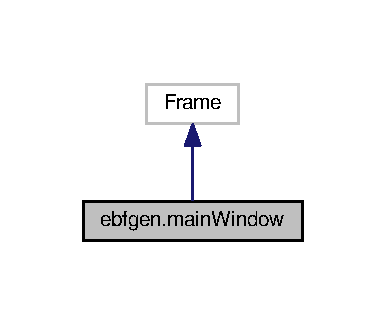
\includegraphics[width=185pt]{classebfgen_1_1mainWindow__inherit__graph}
\end{center}
\end{figure}


Collaboration diagram for ebfgen.\+main\+Window\+:
\nopagebreak
\begin{figure}[H]
\begin{center}
\leavevmode
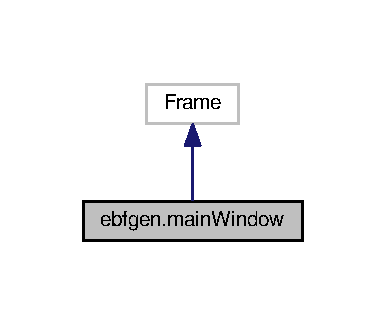
\includegraphics[width=185pt]{classebfgen_1_1mainWindow__coll__graph}
\end{center}
\end{figure}
\subsection*{Public Member Functions}
\begin{DoxyCompactItemize}
\item 
\mbox{\Hypertarget{classebfgen_1_1mainWindow_ac92f39d5be05665356ac78db51336fb6}\label{classebfgen_1_1mainWindow_ac92f39d5be05665356ac78db51336fb6}} 
def {\bfseries \+\_\+\+\_\+init\+\_\+\+\_\+} (self, master=None)
\item 
def \hyperlink{classebfgen_1_1mainWindow_adef0b170df57fd1be0cca767f90e75d9}{clr\+Frame} (self)
\begin{DoxyCompactList}\small\item\em Clear Frame. \end{DoxyCompactList}\item 
def \hyperlink{classebfgen_1_1mainWindow_a7422402e0cb017bfc763f23e448fb966}{rsp\+Update} (self, l)
\begin{DoxyCompactList}\small\item\em Update Frame. \end{DoxyCompactList}\item 
def \hyperlink{classebfgen_1_1mainWindow_ad6fe59c3a2a9e762160dd80263d52f9b}{s\+Std\+V\+A\+Win} (self)
\begin{DoxyCompactList}\small\item\em Start Standard \hyperlink{classebfgen_1_1VA}{VA} Window. \end{DoxyCompactList}\item 
def \hyperlink{classebfgen_1_1mainWindow_a95a4973e95a3ca29f3d4a39aaf0d0aa0}{s\+VE} (self)
\begin{DoxyCompactList}\small\item\em Save VE. \end{DoxyCompactList}\item 
def \hyperlink{classebfgen_1_1mainWindow_a788d4b2795b776cc1cf98e8f1595d919}{upd\+VE} (self)
\begin{DoxyCompactList}\small\item\em Update V\+EC. \end{DoxyCompactList}\item 
def \hyperlink{classebfgen_1_1mainWindow_a062c7d1268146c82264a87132c0f4265}{upd\+VA} ()
\begin{DoxyCompactList}\small\item\em Update \hyperlink{classebfgen_1_1VA}{VA}. \end{DoxyCompactList}\item 
\mbox{\Hypertarget{classebfgen_1_1mainWindow_a9b0a26a4f44410c80e406846ed4ae1de}\label{classebfgen_1_1mainWindow_a9b0a26a4f44410c80e406846ed4ae1de}} 
def \hyperlink{classebfgen_1_1mainWindow_a9b0a26a4f44410c80e406846ed4ae1de}{exit\+Program} (self)
\begin{DoxyCompactList}\small\item\em Quit. \end{DoxyCompactList}\end{DoxyCompactItemize}
\subsection*{Public Attributes}
\begin{DoxyCompactItemize}
\item 
\mbox{\Hypertarget{classebfgen_1_1mainWindow_a3b23dbd8f062622dc6441918fcbdf27c}\label{classebfgen_1_1mainWindow_a3b23dbd8f062622dc6441918fcbdf27c}} 
{\bfseries master}
\item 
\mbox{\Hypertarget{classebfgen_1_1mainWindow_af5ff809c5fc532eee2be62d0539dda15}\label{classebfgen_1_1mainWindow_af5ff809c5fc532eee2be62d0539dda15}} 
{\bfseries l\+\_\+\+V\+EC}
\item 
\mbox{\Hypertarget{classebfgen_1_1mainWindow_a5ff254eceda8c7c130f627d638a9bcf3}\label{classebfgen_1_1mainWindow_a5ff254eceda8c7c130f627d638a9bcf3}} 
{\bfseries l\+\_\+sess}
\item 
\mbox{\Hypertarget{classebfgen_1_1mainWindow_a2cba34bc43b76875e72209d672e77927}\label{classebfgen_1_1mainWindow_a2cba34bc43b76875e72209d672e77927}} 
{\bfseries l\+\_\+city}
\item 
\mbox{\Hypertarget{classebfgen_1_1mainWindow_a9ef3c92baa5e4774182b59f814bdf94e}\label{classebfgen_1_1mainWindow_a9ef3c92baa5e4774182b59f814bdf94e}} 
{\bfseries l\+\_\+state}
\item 
\mbox{\Hypertarget{classebfgen_1_1mainWindow_afcad288db25a2afb1e5428fcbe5eb59e}\label{classebfgen_1_1mainWindow_afcad288db25a2afb1e5428fcbe5eb59e}} 
{\bfseries l\+\_\+appT}
\item 
\mbox{\Hypertarget{classebfgen_1_1mainWindow_af57f2be4222eed2b827e65d469a380e8}\label{classebfgen_1_1mainWindow_af57f2be4222eed2b827e65d469a380e8}} 
{\bfseries l\+\_\+appP}
\item 
\mbox{\Hypertarget{classebfgen_1_1mainWindow_ad0e8ddb1798cc2794366f8035105c942}\label{classebfgen_1_1mainWindow_ad0e8ddb1798cc2794366f8035105c942}} 
{\bfseries l\+\_\+appF}
\item 
\mbox{\Hypertarget{classebfgen_1_1mainWindow_aa96e8be7b03b555b1dc8bae5fb4a194e}\label{classebfgen_1_1mainWindow_aa96e8be7b03b555b1dc8bae5fb4a194e}} 
{\bfseries l\+\_\+elmP}
\item 
\mbox{\Hypertarget{classebfgen_1_1mainWindow_ab82b698d57a7999a62facb332c1207cf}\label{classebfgen_1_1mainWindow_ab82b698d57a7999a62facb332c1207cf}} 
{\bfseries l\+\_\+elmF}
\item 
\mbox{\Hypertarget{classebfgen_1_1mainWindow_ae9c84bd0f4ffd8f96040f090adc3de0a}\label{classebfgen_1_1mainWindow_ae9c84bd0f4ffd8f96040f090adc3de0a}} 
{\bfseries l\+\_\+tloc}
\item 
\mbox{\Hypertarget{classebfgen_1_1mainWindow_a1d5a1a76eedd95c0574ba918fa1ffca3}\label{classebfgen_1_1mainWindow_a1d5a1a76eedd95c0574ba918fa1ffca3}} 
{\bfseries l\+\_\+\+V\+Acnt}
\item 
\mbox{\Hypertarget{classebfgen_1_1mainWindow_a21cbe302421fa6484a061a24b2ab550c}\label{classebfgen_1_1mainWindow_a21cbe302421fa6484a061a24b2ab550c}} 
{\bfseries new\+Window}
\item 
\mbox{\Hypertarget{classebfgen_1_1mainWindow_acdbedb4d27f675dc19bb2b654a29bf7b}\label{classebfgen_1_1mainWindow_acdbedb4d27f675dc19bb2b654a29bf7b}} 
{\bfseries app}
\item 
\mbox{\Hypertarget{classebfgen_1_1mainWindow_afc11b9ae734a3ad4ed3fc5ddb395c1b0}\label{classebfgen_1_1mainWindow_afc11b9ae734a3ad4ed3fc5ddb395c1b0}} 
{\bfseries e\+\_\+\+V\+EC}
\item 
\mbox{\Hypertarget{classebfgen_1_1mainWindow_af681d3309ef2394b44eed26e100b39ed}\label{classebfgen_1_1mainWindow_af681d3309ef2394b44eed26e100b39ed}} 
{\bfseries e\+\_\+sess}
\item 
\mbox{\Hypertarget{classebfgen_1_1mainWindow_aa25e18731405bf2ec08a70145974c63a}\label{classebfgen_1_1mainWindow_aa25e18731405bf2ec08a70145974c63a}} 
{\bfseries e\+\_\+vecity}
\item 
\mbox{\Hypertarget{classebfgen_1_1mainWindow_a43caaec9220c152f68622e8fae62c750}\label{classebfgen_1_1mainWindow_a43caaec9220c152f68622e8fae62c750}} 
{\bfseries e\+\_\+vestate}
\item 
\mbox{\Hypertarget{classebfgen_1_1mainWindow_aa61d58e2a3ac977c0426fa80104eb806}\label{classebfgen_1_1mainWindow_aa61d58e2a3ac977c0426fa80104eb806}} 
{\bfseries e\+\_\+appT}
\item 
\mbox{\Hypertarget{classebfgen_1_1mainWindow_ac3786876d3b6a067f786bd0154996cff}\label{classebfgen_1_1mainWindow_ac3786876d3b6a067f786bd0154996cff}} 
{\bfseries e\+\_\+appP}
\item 
\mbox{\Hypertarget{classebfgen_1_1mainWindow_a5a89ab235f0eedbb6962cb7bd0652e2b}\label{classebfgen_1_1mainWindow_a5a89ab235f0eedbb6962cb7bd0652e2b}} 
{\bfseries e\+\_\+appF}
\item 
\mbox{\Hypertarget{classebfgen_1_1mainWindow_a76e004cd4689514e76a3ef0661549ca3}\label{classebfgen_1_1mainWindow_a76e004cd4689514e76a3ef0661549ca3}} 
{\bfseries e\+\_\+elmP}
\item 
\mbox{\Hypertarget{classebfgen_1_1mainWindow_ae0328da66ac700e30281ac4ecea832a1}\label{classebfgen_1_1mainWindow_ae0328da66ac700e30281ac4ecea832a1}} 
{\bfseries e\+\_\+elmF}
\item 
\mbox{\Hypertarget{classebfgen_1_1mainWindow_a19aab55451fd623e4ee36ded8b13011d}\label{classebfgen_1_1mainWindow_a19aab55451fd623e4ee36ded8b13011d}} 
{\bfseries e\+\_\+tloc}
\item 
\mbox{\Hypertarget{classebfgen_1_1mainWindow_a7da567e81f956f064f718e6bd203114c}\label{classebfgen_1_1mainWindow_a7da567e81f956f064f718e6bd203114c}} 
{\bfseries e\+\_\+tcnt}
\end{DoxyCompactItemize}


\subsection{Detailed Description}
\hyperlink{classebfgen_1_1mainWindow}{main\+Window} Class 

This class represents the main navigation window for ebfgen. Its only real purpose is to provide navigation for the user. 

\subsection{Member Function Documentation}
\mbox{\Hypertarget{classebfgen_1_1mainWindow_adef0b170df57fd1be0cca767f90e75d9}\label{classebfgen_1_1mainWindow_adef0b170df57fd1be0cca767f90e75d9}} 
\index{ebfgen\+::main\+Window@{ebfgen\+::main\+Window}!clr\+Frame@{clr\+Frame}}
\index{clr\+Frame@{clr\+Frame}!ebfgen\+::main\+Window@{ebfgen\+::main\+Window}}
\subsubsection{\texorpdfstring{clr\+Frame()}{clrFrame()}}
{\footnotesize\ttfamily def ebfgen.\+main\+Window.\+clr\+Frame (\begin{DoxyParamCaption}\item[{}]{self }\end{DoxyParamCaption})}



Clear Frame. 

Clears the preview frame. \mbox{\Hypertarget{classebfgen_1_1mainWindow_a7422402e0cb017bfc763f23e448fb966}\label{classebfgen_1_1mainWindow_a7422402e0cb017bfc763f23e448fb966}} 
\index{ebfgen\+::main\+Window@{ebfgen\+::main\+Window}!rsp\+Update@{rsp\+Update}}
\index{rsp\+Update@{rsp\+Update}!ebfgen\+::main\+Window@{ebfgen\+::main\+Window}}
\subsubsection{\texorpdfstring{rsp\+Update()}{rspUpdate()}}
{\footnotesize\ttfamily def ebfgen.\+main\+Window.\+rsp\+Update (\begin{DoxyParamCaption}\item[{}]{self,  }\item[{}]{l }\end{DoxyParamCaption})}



Update Frame. 

Originally for response file previews. Updates the file preview frame \mbox{\Hypertarget{classebfgen_1_1mainWindow_ad6fe59c3a2a9e762160dd80263d52f9b}\label{classebfgen_1_1mainWindow_ad6fe59c3a2a9e762160dd80263d52f9b}} 
\index{ebfgen\+::main\+Window@{ebfgen\+::main\+Window}!s\+Std\+V\+A\+Win@{s\+Std\+V\+A\+Win}}
\index{s\+Std\+V\+A\+Win@{s\+Std\+V\+A\+Win}!ebfgen\+::main\+Window@{ebfgen\+::main\+Window}}
\subsubsection{\texorpdfstring{s\+Std\+V\+A\+Win()}{sStdVAWin()}}
{\footnotesize\ttfamily def ebfgen.\+main\+Window.\+s\+Std\+V\+A\+Win (\begin{DoxyParamCaption}\item[{}]{self }\end{DoxyParamCaption})}



Start Standard \hyperlink{classebfgen_1_1VA}{VA} Window. 

Begins the \char`\"{}standard\char`\"{} Applicant window. \mbox{\Hypertarget{classebfgen_1_1mainWindow_a95a4973e95a3ca29f3d4a39aaf0d0aa0}\label{classebfgen_1_1mainWindow_a95a4973e95a3ca29f3d4a39aaf0d0aa0}} 
\index{ebfgen\+::main\+Window@{ebfgen\+::main\+Window}!s\+VE@{s\+VE}}
\index{s\+VE@{s\+VE}!ebfgen\+::main\+Window@{ebfgen\+::main\+Window}}
\subsubsection{\texorpdfstring{s\+V\+E()}{sVE()}}
{\footnotesize\ttfamily def ebfgen.\+main\+Window.\+s\+VE (\begin{DoxyParamCaption}\item[{}]{self }\end{DoxyParamCaption})}



Save VE. 

Saves V\+EC (Exam) data for the E\+BF header, and prints to the file preview. Note -\/ no matter how many entries are in the preview pane, only one (1) VE record will be in the output. \mbox{\Hypertarget{classebfgen_1_1mainWindow_a062c7d1268146c82264a87132c0f4265}\label{classebfgen_1_1mainWindow_a062c7d1268146c82264a87132c0f4265}} 
\index{ebfgen\+::main\+Window@{ebfgen\+::main\+Window}!upd\+VA@{upd\+VA}}
\index{upd\+VA@{upd\+VA}!ebfgen\+::main\+Window@{ebfgen\+::main\+Window}}
\subsubsection{\texorpdfstring{upd\+V\+A()}{updVA()}}
{\footnotesize\ttfamily def ebfgen.\+main\+Window.\+upd\+VA (\begin{DoxyParamCaption}{ }\end{DoxyParamCaption})}



Update \hyperlink{classebfgen_1_1VA}{VA}. 

Updates the preview pane with the most recently added applicant record. \mbox{\Hypertarget{classebfgen_1_1mainWindow_a788d4b2795b776cc1cf98e8f1595d919}\label{classebfgen_1_1mainWindow_a788d4b2795b776cc1cf98e8f1595d919}} 
\index{ebfgen\+::main\+Window@{ebfgen\+::main\+Window}!upd\+VE@{upd\+VE}}
\index{upd\+VE@{upd\+VE}!ebfgen\+::main\+Window@{ebfgen\+::main\+Window}}
\subsubsection{\texorpdfstring{upd\+V\+E()}{updVE()}}
{\footnotesize\ttfamily def ebfgen.\+main\+Window.\+upd\+VE (\begin{DoxyParamCaption}\item[{}]{self }\end{DoxyParamCaption})}



Update V\+EC. 

Subwindow to update VE header row information for the session. 

The documentation for this class was generated from the following file\+:\begin{DoxyCompactItemize}
\item 
ebfgen.\+py\end{DoxyCompactItemize}

\hypertarget{classebfgen_1_1VA}{}\section{ebfgen.\+VA Class Reference}
\label{classebfgen_1_1VA}\index{ebfgen.\+VA@{ebfgen.\+VA}}


\hyperlink{classebfgen_1_1VA}{VA} Class.  


\subsection*{Public Member Functions}
\begin{DoxyCompactItemize}
\item 
\mbox{\Hypertarget{classebfgen_1_1VA_a47a6dc2f120bc59eed863399f6d57907}\label{classebfgen_1_1VA_a47a6dc2f120bc59eed863399f6d57907}} 
def {\bfseries \+\_\+\+\_\+init\+\_\+\+\_\+} (self, fn, call, ssn, entname, fname, mi, lname, nmsuf, attn, street, pobox, city, state, zipcd, phone, fax, email, appcd, opclass, sigok, physcert, reqexp, waivereq, att, updcall, trusteecall, apptyp, frn, dob, lnchg, psqcd, psq, psqa, felon)
\end{DoxyCompactItemize}
\subsection*{Public Attributes}
\begin{DoxyCompactItemize}
\item 
\mbox{\Hypertarget{classebfgen_1_1VA_a242048a905abbad64a6447cbb9ccb088}\label{classebfgen_1_1VA_a242048a905abbad64a6447cbb9ccb088}} 
{\bfseries fn}
\item 
\mbox{\Hypertarget{classebfgen_1_1VA_a64dc8d7816016b9030d24c9505501809}\label{classebfgen_1_1VA_a64dc8d7816016b9030d24c9505501809}} 
{\bfseries call}
\item 
\mbox{\Hypertarget{classebfgen_1_1VA_ae669bff80f0ac4f4df796ae207297e4e}\label{classebfgen_1_1VA_ae669bff80f0ac4f4df796ae207297e4e}} 
{\bfseries ssn}
\item 
\mbox{\Hypertarget{classebfgen_1_1VA_a240ae8d4fc4684a5cb961c15fd1637ce}\label{classebfgen_1_1VA_a240ae8d4fc4684a5cb961c15fd1637ce}} 
{\bfseries entname}
\item 
\mbox{\Hypertarget{classebfgen_1_1VA_a403d62aea2916b58f63d562ca2e89c37}\label{classebfgen_1_1VA_a403d62aea2916b58f63d562ca2e89c37}} 
{\bfseries fname}
\item 
\mbox{\Hypertarget{classebfgen_1_1VA_a8fd3ae605906303bcb9ff76eccccec7f}\label{classebfgen_1_1VA_a8fd3ae605906303bcb9ff76eccccec7f}} 
{\bfseries mi}
\item 
\mbox{\Hypertarget{classebfgen_1_1VA_a68d13369f268c1491eca7cea2c105e4b}\label{classebfgen_1_1VA_a68d13369f268c1491eca7cea2c105e4b}} 
{\bfseries lname}
\item 
\mbox{\Hypertarget{classebfgen_1_1VA_aa305da8d39c58a7695d18721176227e5}\label{classebfgen_1_1VA_aa305da8d39c58a7695d18721176227e5}} 
{\bfseries nmsuf}
\item 
\mbox{\Hypertarget{classebfgen_1_1VA_a20754776f4778eca87243a140155e18f}\label{classebfgen_1_1VA_a20754776f4778eca87243a140155e18f}} 
{\bfseries attn}
\item 
\mbox{\Hypertarget{classebfgen_1_1VA_ad458bdf0498989ff9d2c891f2015e52a}\label{classebfgen_1_1VA_ad458bdf0498989ff9d2c891f2015e52a}} 
{\bfseries street}
\item 
\mbox{\Hypertarget{classebfgen_1_1VA_af6121ad445c3455d6fe3480964b8dc3a}\label{classebfgen_1_1VA_af6121ad445c3455d6fe3480964b8dc3a}} 
{\bfseries pobox}
\item 
\mbox{\Hypertarget{classebfgen_1_1VA_a264eca9621b5365c4ce4f084b3a14076}\label{classebfgen_1_1VA_a264eca9621b5365c4ce4f084b3a14076}} 
{\bfseries city}
\item 
\mbox{\Hypertarget{classebfgen_1_1VA_a088beb68a7f6b1c8005fc156bab6f170}\label{classebfgen_1_1VA_a088beb68a7f6b1c8005fc156bab6f170}} 
{\bfseries state}
\item 
\mbox{\Hypertarget{classebfgen_1_1VA_a6152d925e20e9e4ae2942ea1eee4bca9}\label{classebfgen_1_1VA_a6152d925e20e9e4ae2942ea1eee4bca9}} 
{\bfseries zipcd}
\item 
\mbox{\Hypertarget{classebfgen_1_1VA_ae339e8e8c7d54ad55acb903dfa0a04eb}\label{classebfgen_1_1VA_ae339e8e8c7d54ad55acb903dfa0a04eb}} 
{\bfseries phone}
\item 
\mbox{\Hypertarget{classebfgen_1_1VA_a7571a738bde29a57880c794a8509c3a1}\label{classebfgen_1_1VA_a7571a738bde29a57880c794a8509c3a1}} 
{\bfseries fax}
\item 
\mbox{\Hypertarget{classebfgen_1_1VA_ab777b2f8a3cf7e486f57edecd7b9bcc3}\label{classebfgen_1_1VA_ab777b2f8a3cf7e486f57edecd7b9bcc3}} 
{\bfseries email}
\item 
\mbox{\Hypertarget{classebfgen_1_1VA_a0680a9485123820c559ab15ce9ede290}\label{classebfgen_1_1VA_a0680a9485123820c559ab15ce9ede290}} 
{\bfseries appcd}
\item 
\mbox{\Hypertarget{classebfgen_1_1VA_ae9433cf523f21ae9d5b8374233aa2e19}\label{classebfgen_1_1VA_ae9433cf523f21ae9d5b8374233aa2e19}} 
{\bfseries opclass}
\item 
\mbox{\Hypertarget{classebfgen_1_1VA_a65f1f3767164e954c077a49db91bb376}\label{classebfgen_1_1VA_a65f1f3767164e954c077a49db91bb376}} 
{\bfseries sigok}
\item 
\mbox{\Hypertarget{classebfgen_1_1VA_a3b8a3d38e455da340ccd63c34311763f}\label{classebfgen_1_1VA_a3b8a3d38e455da340ccd63c34311763f}} 
{\bfseries physcert}
\item 
\mbox{\Hypertarget{classebfgen_1_1VA_adabae22f328382300efdc64f9471a431}\label{classebfgen_1_1VA_adabae22f328382300efdc64f9471a431}} 
{\bfseries reqexp}
\item 
\mbox{\Hypertarget{classebfgen_1_1VA_a87b4afed0fb8b37476b27baddf220115}\label{classebfgen_1_1VA_a87b4afed0fb8b37476b27baddf220115}} 
{\bfseries waivereq}
\item 
\mbox{\Hypertarget{classebfgen_1_1VA_a91d54b64a33d0edc7e724dc111f4647d}\label{classebfgen_1_1VA_a91d54b64a33d0edc7e724dc111f4647d}} 
{\bfseries att}
\item 
\mbox{\Hypertarget{classebfgen_1_1VA_afc1dc5ebaf567de5c37ff9622bf5caf2}\label{classebfgen_1_1VA_afc1dc5ebaf567de5c37ff9622bf5caf2}} 
{\bfseries updcall}
\item 
\mbox{\Hypertarget{classebfgen_1_1VA_ae3b1f91f5cd80a96aa476a4aef1ab59c}\label{classebfgen_1_1VA_ae3b1f91f5cd80a96aa476a4aef1ab59c}} 
{\bfseries trusteecall}
\item 
\mbox{\Hypertarget{classebfgen_1_1VA_a842c14650ed01ec55cf408c8103caf25}\label{classebfgen_1_1VA_a842c14650ed01ec55cf408c8103caf25}} 
{\bfseries apptyp}
\item 
\mbox{\Hypertarget{classebfgen_1_1VA_aac8ec55be3de85f83331d34b1ffbc9a2}\label{classebfgen_1_1VA_aac8ec55be3de85f83331d34b1ffbc9a2}} 
{\bfseries frn}
\item 
\mbox{\Hypertarget{classebfgen_1_1VA_ae82a18287640edf9a020e85939925036}\label{classebfgen_1_1VA_ae82a18287640edf9a020e85939925036}} 
{\bfseries dob}
\item 
\mbox{\Hypertarget{classebfgen_1_1VA_a07a5f205dbdc509a88865d8e22c61c87}\label{classebfgen_1_1VA_a07a5f205dbdc509a88865d8e22c61c87}} 
{\bfseries lnchg}
\item 
\mbox{\Hypertarget{classebfgen_1_1VA_a90c902db56a8a396d99eebdf67fda4d6}\label{classebfgen_1_1VA_a90c902db56a8a396d99eebdf67fda4d6}} 
{\bfseries psqcd}
\item 
\mbox{\Hypertarget{classebfgen_1_1VA_a28551d85cb13f759880c76926876c01e}\label{classebfgen_1_1VA_a28551d85cb13f759880c76926876c01e}} 
{\bfseries psq}
\item 
\mbox{\Hypertarget{classebfgen_1_1VA_acb3e7be0b59346ca415bac320fac379b}\label{classebfgen_1_1VA_acb3e7be0b59346ca415bac320fac379b}} 
{\bfseries psqa}
\item 
\mbox{\Hypertarget{classebfgen_1_1VA_a1e1da0cbed7cd1cbfb227b4b1c893f24}\label{classebfgen_1_1VA_a1e1da0cbed7cd1cbfb227b4b1c893f24}} 
{\bfseries felon}
\end{DoxyCompactItemize}


\subsection{Detailed Description}
\hyperlink{classebfgen_1_1VA}{VA} Class. 

The \char`\"{}\+V\+A\char`\"{} class object maintains the details of an individual applicant for a given testing session. At the present time, pyebfgen does not support editing of applicant data once saved. 

The documentation for this class was generated from the following file\+:\begin{DoxyCompactItemize}
\item 
ebfgen.\+py\end{DoxyCompactItemize}

%--- End generated contents ---

% Index
\backmatter
\newpage
\phantomsection
\clearemptydoublepage
\addcontentsline{toc}{chapter}{Index}
\printindex

\end{document}
